% A0 portrait poster -- petrol + copper palette, sections with subsections.
% Compile with XeLaTeX or LuaLaTeX:  latexmk -xelatex poster_portrait.tex
\documentclass{article}
\usepackage[paperwidth=84.1cm,paperheight=118.9cm,
            left=2.2cm,right=2.2cm,top=10.5cm,bottom=4.2cm]{geometry}
\usepackage{fontspec}
\usepackage{amsmath,amssymb}
\usepackage{xcolor}
\usepackage{tikz}
\usetikzlibrary{calc}
\usepackage[most]{tcolorbox}
\usepackage{enumitem}
\usepackage{microtype}
\usepackage{graphicx}

\IfFontExistsTF{Arial}{\setmainfont{Arial}}{\setmainfont{Liberation Sans}}
\pagestyle{empty}
\setlength{\parindent}{0pt}
\setlength{\parskip}{0.38em}
\setlist[itemize]{leftmargin=1.1em,itemsep=0.18em,topsep=0.25em,parsep=0pt}

% ---------------------------------------------------------------- palette
\definecolor{Petrol}{HTML}{123B4A}      % header, section bars
\definecolor{PetrolDeep}{HTML}{0C2A35}  % take-home band
\definecolor{Copper}{HTML}{D0703C}      % single accent
\definecolor{CopperPale}{HTML}{FBEDE4}  % claim background
\definecolor{PetrolPale}{HTML}{E4EDEF}  % secondary highlight
\definecolor{Paper}{HTML}{F4F6F5}
\definecolor{Ink}{HTML}{1E2A30}
\definecolor{Mid}{HTML}{66747A}
\definecolor{Rule}{HTML}{CFD8DA}
\definecolor{Placeholder}{HTML}{E9EDEC}
% variable colours (kept distinct from the frame colours)
\definecolor{Ucol}{HTML}{C61826}  % activator
\definecolor{Vcol}{HTML}{0072B2}  % inhibitor
\definecolor{Rcol}{HTML}{7B4FA0}  % source density

\newcommand{\U}{\textcolor{Ucol}{u}}
\newcommand{\V}{\textcolor{Vcol}{v}}
\newcommand{\R}{\textcolor{Rcol}{\rho}}

\color{Ink}
\newcommand{\bodyfont}{\fontsize{22}{27.5}\selectfont}
\newcommand{\smallfont}{\fontsize{19}{23.5}\selectfont}
\newcommand{\tinyfont}{\fontsize{14}{17}\selectfont}
\newcommand{\eqnfont}{\fontsize{22}{28}\selectfont}
\newcommand{\placeholderfont}{\fontsize{19}{23}\selectfont\bfseries\color{Mid}}

% ---------------------------------------------------------------- layout
\newlength{\colw}\setlength{\colw}{38.6cm}
\newlength{\secgap}\setlength{\secgap}{1.1cm}

% full-width section bar
\newcommand{\postersection}[2]{%
  \par\noindent
  \begin{tikzpicture}
    \fill[Petrol,rounded corners=3mm] (0,0) rectangle (\linewidth,2.4cm);
    \node[anchor=west,text=white,font=\fontsize{36}{40}\selectfont\bfseries]
      at (1.0cm,1.2cm) {\textcolor{Copper}{#1}\hspace{0.7em}#2};
  \end{tikzpicture}\par\vspace{0.5cm}%
}

% subsection heading inside a column
\newcommand{\postersub}[2]{%
  \par\vspace{0.5cm}\noindent
  {\fontsize{27}{31}\selectfont\bfseries\color{Copper}#1\hspace{0.45em}\color{Petrol}#2}\par
  \vspace{-0.2cm}\noindent{\color{Copper}\rule{\linewidth}{1.6pt}}\par\vspace{0.1cm}%
}

\newcommand{\placeholder}[2]{%
  \par\noindent
  \begin{tikzpicture}
    \node[draw=Mid,dashed,line width=1.4pt,rounded corners=3mm,fill=Placeholder,
          minimum width=\linewidth,minimum height=#1,text width=0.85\linewidth,
          align=center,inner sep=0pt] {\placeholderfont #2};
  \end{tikzpicture}\par
}

\newcommand{\claim}[1]{%
  \begin{tcolorbox}[enhanced,colback=CopperPale,colframe=Copper,boxrule=1.4pt,arc=3mm,
                    left=7mm,right=7mm,top=4mm,bottom=4mm,before skip=0.45cm,after skip=0.1cm]
  \fontsize{26}{32}\selectfont\bfseries\color{Petrol}#1
  \end{tcolorbox}%
}

\newcommand{\note}[1]{%
  \begin{tcolorbox}[colback=PetrolPale,colframe=PetrolPale,boxrule=0pt,arc=2mm,
                    left=5mm,right=5mm,top=3mm,bottom=3mm,before skip=0.4cm,after skip=0.2cm]
  \fontsize{20}{25}\selectfont\bfseries\color{Petrol}#1
  \end{tcolorbox}%
}

\newcommand{\minitag}[1]{\tikz[baseline=(X.base)]\node[fill=PetrolPale,rounded corners=2mm,
    inner xsep=3mm,inner ysep=1.5mm,text=Petrol,font=\fontsize{17}{19}\selectfont\bfseries] (X) {#1};}

\newenvironment{leftcol}{\begin{minipage}[t]{\colw}\bodyfont}{\end{minipage}\hfill}
\newenvironment{rightcol}{\begin{minipage}[t]{\colw}\bodyfont}{\end{minipage}}

% ================================================================ document
\begin{document}
\begin{tikzpicture}[remember picture,overlay]
  \fill[Paper] (current page.south west) rectangle (current page.north east);
  % header
  \fill[Petrol] (current page.north west) rectangle ([yshift=-9.0cm]current page.north east);
  \fill[Copper] ([yshift=-9.0cm]current page.north west) rectangle ([yshift=-9.4cm]current page.north east);
  \node[anchor=north west,inner sep=0pt,text width=57cm,text=white,
        align=left,font=\fontsize{56}{64}\selectfont\bfseries] (title)
    at ([xshift=2.2cm,yshift=-1.3cm]current page.north west)
    {What Does Source Density Add to Models of\\Hydra Patterning and Regeneration?};
  \node[anchor=north west,inner sep=0pt,text width=57cm,text=white,
        font=\fontsize{25}{31}\selectfont] (authors)
    at ([yshift=-0.9cm]title.south west)
    {Szymon~Cygan \quad\textperiodcentered\quad Anna~Marciniak-Czochra
     \quad\textperiodcentered\quad Finn~Münnich \quad\textperiodcentered\quad Moritz~Mercker};
  \node[anchor=north west,inner sep=0pt,text width=57cm,text=white!75!Petrol,
        font=\fontsize{20}{25}\selectfont]
    at ([yshift=-0.35cm]authors.south west)
    {Heidelberg University, Heidelberg, Germany};
  \node[anchor=north east,fill=white,rounded corners=4mm,inner sep=6mm]
    at ([xshift=-2.2cm,yshift=-1.6cm]current page.north east)
    {
\includegraphics[height=5.0cm]{assets/heidelberg_logo.png}};
  % footer
  \fill[white] (current page.south west) rectangle ([yshift=3.4cm]current page.south east);
  \fill[Copper] ([yshift=3.4cm]current page.south west) rectangle ([yshift=3.6cm]current page.south east);
  \node[anchor=west,inner sep=0pt,text width=60cm,font=\tinyfont]
    at ([xshift=2.2cm,yshift=1.7cm]current page.south west) {\color{Mid}
      \textbf{\color{Petrol}Selected references:} Gierer \& Meinhardt, \textit{Kybernetik} 12 (1972), 30--39.
      Suzuki \& Takagi, \textit{Funkcialaj Ekvacioj} 54 (2011), 237--274.
      Livshits et al., \textit{Scientific Reports} 12 (2022), 13368.};
  \node[anchor=east,inner sep=0pt,align=right]
    at ([xshift=-2.2cm,yshift=1.7cm]current page.south east)
    {\fontsize{16}{19}\selectfont\bfseries\color{Petrol}SFB RETREAT\\[-1mm]
     \mdseries\color{Mid}portrait layout draft};
\end{tikzpicture}%
\noindent
% ================================================================ 1
\postersection{1}{Motivation}
\begin{leftcol}
  \postersub{1.1}{Hydra as a patterning problem}
  \begin{minipage}[t]{8.0cm}\vspace{0pt}
    
\includegraphics[width=\linewidth]{assets/hydra.png}
  \end{minipage}\hfill
  \begin{minipage}[t]{29.6cm}\vspace{0pt}
    A \emph{Hydra} regenerates a single head after amputation and keeps its
    oral--aboral axis. Head formation is organised by a localised
    Wnt/$\beta$-catenin signal.

    \smallfont
    In activator--inhibitor models, the head is represented by a localised
    peak of the activator~\U, controlled by a long-range inhibitor~\V.
  \end{minipage}
\end{leftcol}
\begin{rightcol}
  \postersub{1.2}{Head grafting}
  \placeholder{6.4cm}{HEAD-GRAFT SCHEMATIC\\head tissue transplanted into the body column\\$\rightarrow$ secondary axis, outcome depends on graft position}
  \smallfont
  A grafted head can induce a second axis. Whether it does depends on
  \emph{where} in the host body column it is placed.
\end{rightcol}

\claim{One model must separate three phenomena: regeneration, pattern selection, and positional memory.}

\vspace{\secgap}
% ================================================================ 2
\postersection{2}{What the activator--inhibitor model already does}
\begin{leftcol}
  \postersub{2.1}{Production terms change the phase portrait}
  \eqnfont
  \[
  \begin{aligned}
  \partial_t \U &= D_u\Delta \U + \frac{a \U^2+q_u}{\V}-\mu_u \U+p_u,\\
  \partial_t \V &= D_v\Delta \V + b \U^2-\mu_v \V+p_v.
  \end{aligned}
  \]
  \bodyfont
  The three production terms are not interchangeable:
  \begin{itemize}
    \item $p_v$: basal inhibitor production; regularises the resting state,
    \item $p_u$: external activator input,
    \item $q_u$: activator input inside inhibitor regulation.
  \end{itemize}
  Homogeneous equilibria satisfy the cubic
  \[
  P(u)=\mu_u b u^3-(a\mu_v+b p_u)u^2+\mu_u p_v u-(\mu_v q_u+p_u p_v)=0.
  \]
  \begin{minipage}[t]{21.5cm}\vspace{0pt}
  \placeholder{7.8cm}{PHASE-PORTRAIT PLACEHOLDER\\one vs.\ three homogeneous states\\nullclines + stability markers}
  \end{minipage}\hfill
  \begin{minipage}[t]{16.3cm}\vspace{0pt}\smallfont\setlength{\parskip}{0.55em}
  \minitag{1 state} high activator production can remove the threshold.\par
  \minitag{3 states} lower rest + unstable threshold + upper active state.\par
  \minitag{DII} an outer kinetically stable state can become diffusion unstable.
  \end{minipage}

  \postersub{2.2}{Inhibitor production creates a threshold}
  \begin{minipage}[t]{19.5cm}\vspace{0pt}
  From here on $p_u=q_u=0$:\par
  \eqnfont
  \[
  \begin{aligned}
  \partial_t \U &=D_u\Delta \U+\frac{a \U^2}{\V}-\mu_u \U,\\
  \partial_t \V &=D_v\Delta \V+b \U^2-\mu_v \V+p_v.
  \end{aligned}
  \]
  \end{minipage}\hfill
  \begin{minipage}[t]{18.3cm}\vspace{0pt}\smallfont
  Rest state $E_0=(0,p_v/\mu_v)$. Two positive states $E_\pm$ exist when
  \[
  \Delta_h=a^2\mu_v^2-4\mu_u^2 b p_v>0,
  \]
  \[
  u_{\pm}=\frac{a\mu_v\pm\sqrt{\Delta_h}}{2\mu_u b},
  \quad v_{\pm}=\frac{a}{\mu_u}u_{\pm}.
  \]
  \end{minipage}\par
  \smallfont
  $E_-$ is the activation threshold; $E_+$ is the candidate
  pattern-forming state.
  \note{Basal inhibitor production already gives a stable rest state,
  bistability, and a finite-amplitude trigger.}
\end{leftcol}
\begin{rightcol}
  \postersub{2.3}{Regeneration needs a finite wound}
  \placeholder{6.8cm}{JULIA SIMULATION PLACEHOLDER\\weak versus strong localised perturbation}
  \smallfont
  A weak perturbation returns to rest. A sufficiently strong localised
  perturbation crosses $E_-$ and produces a persistent activator peak.

  \postersub{2.4}{Grafts: the model chooses the position}
  \placeholder{6.8cm}{JULIA SIMULATION PLACEHOLDER\\wound away from preferred position\\transient peak at the wound $\rightarrow$ drift to boundary / middle / one third}
  \smallfont
  A second peak can be initiated by a wound, but its final position is not
  arbitrary: a peak created away from a preferred location drifts to a
  position selected by domain size and unstable modes.

  \postersub{2.5}{Pattern selection depends on history}
  \placeholder{6.8cm}{JULIA SIMULATION PLACEHOLDER\\same final domain, two preparation histories\\direct DII: many peaks \,|\, growth continuation: one peak}
  \smallfont
  Starting near the diffusion-unstable state on a large domain selects
  several peaks. Growing the domain from a small one preserves a single
  established peak in the same final parameter regime.
\end{rightcol}

\claim{Source density is not needed to make a head --- but the model, not the wound, decides where the head ends up.}

\vspace{\secgap}
% ================================================================ 3
\postersection{3}{Positional memory and source density}
\begin{leftcol}
  \postersub{3.1}{Grafting exposes missing information}
  {\centering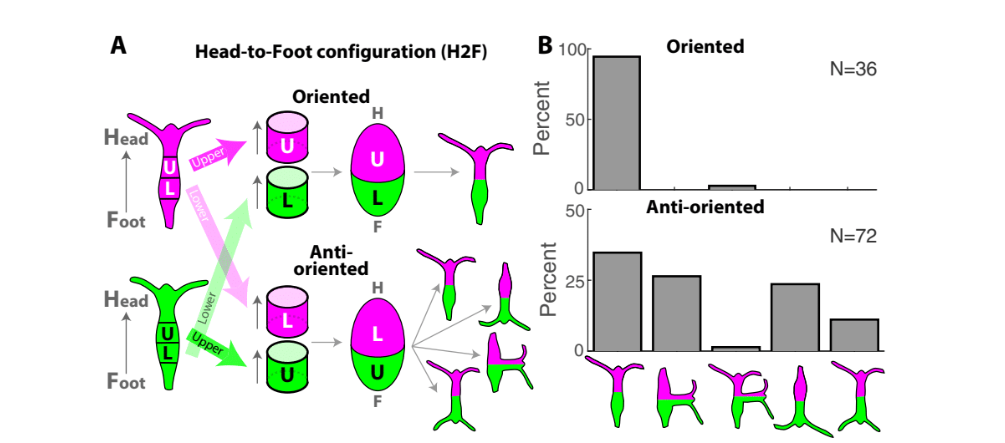
\includegraphics[width=0.86\linewidth]{assets/livshits_h2f_experiment.png}\par}
  {\tinyfont\color{Mid} Head-to-foot grafts, oriented vs.\ anti-oriented. Livshits et al.\ (2022), K.~Keren group.\par}
  \smallfont
  Reversing the orientation of comparable tissue pieces changes the
  distribution of outcomes. Near the resting state, \U\ and \V\ alone do not
  distinguish an upper-body fragment from a lower-body one.
  \note{Which state variable records the original position and orientation of the grafted tissue?}

  \postersub{3.2}{Prescribed $\rho(x)$ as tissue competence}
  \placeholder{4.6cm}{PROFILE PLACEHOLDER\\oriented and anti-oriented piecewise $\rho(x)$}
  \smallfont
  A fixed source-density profile encodes tissue origin before the activator
  is present and biases where a wound-triggered peak forms (source-gradient
  idea, Suzuki \& Takagi 2011).
\end{leftcol}
\begin{rightcol}
  \postersub{3.3}{Dynamic source-density model}
  \eqnfont
  \[
  \begin{aligned}
  \partial_t \U &=D_u\Delta \U+\R\,\frac{a \U^2}{\V}-\mu_u \U,\\
  \partial_t \V &=D_v\Delta \V+b\R\,\U^2-\mu_v \V+p_v,\\
  \tau\,\partial_t\R&=D_\rho\Delta\R+\U-\R.
  \end{aligned}
  \]
  \smallfont
  \begin{itemize}
    \item $\rho(0,x)$ stores the grafted configuration,
    \item $\tau$ sets the lifetime of memory,
    \item $D_\rho$ communicates positional information in space.
  \end{itemize}

  \postersub{3.4}{Dynamic $\rho$ gives metastable memory}
  \placeholder{7.5cm}{JULIA SIMULATION PLACEHOLDER\\long-lived peak near the graft + peak position $x_{\max}(t)$}
  \smallfont
  The inherited $\rho$ profile anchors a peak near the graft on the fast
  \U--\V\ time scale. As $\rho$ relaxes, the peak drifts toward a position
  preferred by the activator--inhibitor subsystem.

  \postersub{3.5}{Diffusion sets the spatial reach of memory}
  \placeholder{4.6cm}{PARAMETER-SWEEP PLACEHOLDER\\memory time versus $D_\rho$ and $\tau$}
  \smallfont
  $D_\rho$ too small: memory stays sharply localised. Intermediate: a usable
  gradient forms. Too large: spatial information is erased.
\end{rightcol}

\claim{Source density can hold positional memory for a long time --- without making the graft-selected peak truly stationary.}

\vspace{\secgap}
% ================================================================ 4
\begin{tcolorbox}[enhanced,colback=PetrolDeep,colframe=PetrolDeep,arc=3mm,
                  left=1.2cm,right=1.2cm,top=0.6cm,bottom=0.6cm,before skip=0pt]
\color{white}
\begin{minipage}[t]{0.52\linewidth}
  {\fontsize{34}{38}\selectfont\bfseries\color{Copper}Take-home message\par}
  \vspace{0.25cm}
  \fontsize{22}{28}\selectfont
  \begin{enumerate}[leftmargin=1.3em,itemsep=0.35em,topsep=0pt]
    \item \textbf{$p_v$ is enough} for a rest state, an activation threshold, and patterning.
    \item \textbf{The model selects head positions}; wounds elsewhere give transient peaks.
    \item \textbf{$\rho$ adds inherited positional information} for grafted tissue.
    \item \textbf{Dynamic $\rho$ gives metastability}: long-lived anchoring, then slow reorganisation.
  \end{enumerate}
\end{minipage}\hfill
\begin{minipage}[t]{0.42\linewidth}
  \vspace{0.3cm}
  {\fontsize{32}{40}\selectfont\bfseries
  Source density is not needed to make a head.\\
  \textcolor{Copper}{It may be needed to remember where a head should form.}\par}
  \vspace{0.5cm}
  {\fontsize{19}{24}\selectfont\color{white!80!PetrolDeep}
  \textbf{\color{white}Outlook.} A non-diffusing head-identity variable $h$
  with hysteresis could separate transient activator peaks from stable
  morphological commitment.\par}
\end{minipage}
\end{tcolorbox}
\end{document}
